%%
%% Copyright 2007, 2008, 2009 Elsevier Ltd
%%
%% This file is part of the 'Elsarticle Bundle'.
%% ---------------------------------------------
%%
%% It may be distributed under the conditions of the LaTeX Project Public
%% License, either version 1.2 of this license or (at your option) any
%% later version.  The latest version of this license is in
%%    http://www.latex-project.org/lppl.txt
%% and version 1.2 or later is part of all distributions of LaTeX
%% version 1999/12/01 or later.
%%
%% The list of all files belonging to the 'Elsarticle Bundle' is
%% given in the file `manifest.txt'.
%%

%% Template article for Elsevier's document class `elsarticle'
%% with numbered style bibliographic references
%% SP 2008/03/01
%%
%%
%%
%% $Id: elsarticle-template-num.tex 4 2009-10-24 08:22:58Z rishi $
%%
%%
%\documentclass[preprint,12pt]{elsarticle}

%% Use the option review to obtain double line spacing
\documentclass[preprint,review,12pt]{elsarticle}

%% Use the options 1p,twocolumn; 3p; 3p,twocolumn; 5p; or 5p,twocolumn
%% for a journal layout:
%% \documentclass[final,1p,times]{elsarticle}
%% \documentclass[final,1p,times,twocolumn]{elsarticle}
%% \documentclass[final,3p,times]{elsarticle}
%% \documentclass[final,3p,times,twocolumn]{elsarticle}
%% \documentclass[final,5p,times]{elsarticle}
%% \documentclass[final,5p,times,twocolumn]{elsarticle}

%% if you use PostScript figures in your article
%% use the graphics package for simple commands
%% \usepackage{graphics}
%% or use the graphicx package for more complicated commands
%% \usepackage{graphicx}
%% or use the epsfig package if you prefer to use the old commands
%% \usepackage{epsfig}
%%%%%%%%%%%%%%%%%%%%%%%%%%%%%%%%%%%%%%%%%%%%%%%%%%%%%%%%%%%%%%%%%%%%
%% Package Listing
\usepackage{color}
\usepackage{graphicx}
\usepackage{amssymb}
\usepackage{amsmath}
\usepackage{amsfonts}
\usepackage{amstext}
\usepackage{amsbsy}
\usepackage{epstopdf}
\usepackage{float}
\usepackage{bigints}
\usepackage{caption}
\usepackage{subcaption}
%%%%%%%%%%%%%%%%%%%%%%%%%%%%%%%%%%%%%%%%%%%%%%%%%%%%%%%%%%%%%%%%%%%%
%% The lineno packages adds line numbers. Start line numbering with
%% \begin{linenumbers}, end it with \end{linenumbers}. Or switch it on
%% for the whole article with \linenumbers after \end{frontmatter}.
\usepackage{lineno}
%%%%%%%%%%%%%%%%%%%%%%%%%%%%%%%%%%%%%%%%%%%%%%%%%%%%%%%%%%%%%%%%%%%%
% DGFEM commands
\newcommand{\jmp}[1]{[\![#1]\!]}                     % jump
\newcommand{\mvl}[1]{\{\!\!\{#1\}\!\!\}}             % mean value
\newcommand{\keff}{\ensuremath{k_{\textit{eff}}}\xspace}
%% Other Commands
\newcommand{\tcr}[1]{\textcolor{red}{#1}}
\newcommand{\mt}[1]{\marginpar{ {\tiny #1}}}
\newcommand{\Introfigpath}[1]{../../../Document/Rev0/figures/sec_Intro/{#1}}
\newcommand{\Snfigpath}[1]{../../../Document/Rev0/figures/sec_Sn/{#1}}
\newcommand{\BFfigpath}[1]{../../../Document/Rev0/figures/sec_BF/{#1}}
\newcommand{\DSAfigpath}[1]{../../../Document/Rev0/figures/sec_DSA/{#1}}
%%%%%%%%%%%%%%%%%%%%%%%%%%%%%%%%%%%%%%%%%%%%%%%%%%%%%%%%%%%%%%%%%%%%
\journal{SIAM Journal on Scientific Computing}

\begin{document}
%-------------------------
\begin{frontmatter}
%-------------------------
\title{Scalable DSA Preconditioner for the DFEM $S_N$ Transport Equation on Massively-Parallel Architectures}
%-------------------------
\author[kapl]{Michael~W.~Hackemack\corref{cor1}}
\ead{michael.hackemack@unnpp.gov}
\author[tamu]{Jean~C.~Ragusa}
\ead{jean.ragusa@tamu.edu}
\address[kapl]{Knolls Atomic Power Laboratory, P.O. Box 1072, Schenectady, NY 12301}
\address[tamu]{Department of Nuclear Engineering, Texas A\&M University, College Station, TX 77843, USA}
\cortext[cor1]{Corresponding author}
%-------------------------
\begin{abstract}
%% Text of abstract

\end{abstract}
%-------------------------
\begin{keyword}
Radiation Transport \sep Scalable \sep Parallel \sep Diffusion Synthetic Acceleration \sep Modified Interior Penalty Method
\end{keyword}
%-------------------------
\end{frontmatter}
%-------------------------
%%%%%%%%%%%%%%%%%%%%%%%%%%%%%%%%%%%%%%%%%%%%%%%%%%%%%%%%%%%%%%%%%%%%

\linenumbers

%%%%%%%%%%%%%%%%%%%%%%%%%%%%%%%%%%%%%%%%%%%%%%%%%%%%%%%%%%%%%%%%%%%%
%%%%%%%%%%%%%%%%%%%%%%%%%%%%%%%%%%%%%%%%%%%%%%%%%%%%%%%%%%%%%%%%%%%%
\section{Introduction} \label{sec::intro}
%%%%%%%%%%%%%%%%%%%%%%%%%%%%%%%%%%%%%%%%%%%%%%%%%%%%%%%%%%%%%%%%%%%%
%%%%%%%%%%%%%%%%%%%%%%%%%%%%%%%%%%%%%%%%%%%%%%%%%%%%%%%%%%%%%%%%%%%%

Intro goes here...

% Outline goes here
%------------------------
The remainder of this paper is outlined as follows. 
%------------------------

%%%%%%%%%%%%%%%%%%%%%%%%%%%%%%%%%%%%%%%%%%%%%%%%%%%%%%%%%%%%%%%%%%%%
%%%%%%%%%%%%%%%%%%%%%%%%%%%%%%%%%%%%%%%%%%%%%%%%%%%%%%%%%%%%%%%%%%%%
\section{The First-Order Form of the Transport Equation} \label{sec::trans}
%%%%%%%%%%%%%%%%%%%%%%%%%%%%%%%%%%%%%%%%%%%%%%%%%%%%%%%%%%%%%%%%%%%%
%%%%%%%%%%%%%%%%%%%%%%%%%%%%%%%%%%%%%%%%%%%%%%%%%%%%%%%%%%%%%%%%%%%%

%------------------------------------------------------------------------------------------------------------
\subsection{The DFEM $S_N$ Transport Equation} \label{sec::trans_DFEMSn}
%------------------------------------------------------------------------------------------------------------

% Look at Bruno's MIP paper here
% 1) start with continuous equation with isotropic source and scattering
% 2) 
% 3) 


%------------------------------------------------------------------------------------------------------------
\subsection{Solving with a Richardson Iteration Scheme} \label{sec::trans_SI}
%------------------------------------------------------------------------------------------------------------

% 1) operator notation from previous section to define SI

%%%%%%%%%%%%%%%%%%%%%%%%%%%%%%%%%%%%%%%%%%%%%%%%%%%%%%%%%%%%%%%%%%%%
%%%%%%%%%%%%%%%%%%%%%%%%%%%%%%%%%%%%%%%%%%%%%%%%%%%%%%%%%%%%%%%%%%%%
\section{Inverting the Loss Operator - The $S_N$ Transport Sweep} \label{sec::sweep}
%%%%%%%%%%%%%%%%%%%%%%%%%%%%%%%%%%%%%%%%%%%%%%%%%%%%%%%%%%%%%%%%%%%%
%%%%%%%%%%%%%%%%%%%%%%%%%%%%%%%%%%%%%%%%%%%%%%%%%%%%%%%%%%%%%%%%%%%%



%%%%%%%%%%%%%%%%%%%%%%%%%%%%%%%%%%%%%%%%%%%%%%%%%%%%%%%%%%%%%%%%%%%%
%%%%%%%%%%%%%%%%%%%%%%%%%%%%%%%%%%%%%%%%%%%%%%%%%%%%%%%%%%%%%%%%%%%%
\section{Preconditioning by Synthetic Acceleration} \label{sec::accel}
%%%%%%%%%%%%%%%%%%%%%%%%%%%%%%%%%%%%%%%%%%%%%%%%%%%%%%%%%%%%%%%%%%%%
%%%%%%%%%%%%%%%%%%%%%%%%%%%%%%%%%%%%%%%%%%%%%%%%%%%%%%%%%%%%%%%%%%%%

% Discuss overview of synthetic acceleration
% 1) formulation to get to low-order operator
% 2) mention that we will use DSA
% 3) mention particular DSA is MIP (with section mention)

%------------------------------------------------------------------------------------------------------------
\subsection{Diffusion Synthetic Acceleration} \label{sec::accel_DSA}
%------------------------------------------------------------------------------------------------------------

%------------------------------------------------------------------------------------------------------------
\subsection{The Modified Interior Penalty Method} \label{sec::accel_MIP}
%------------------------------------------------------------------------------------------------------------



%%%%%%%%%%%%%%%%%%%%%%%%%%%%%%%%%%%%%%%%%%%%%%%%%%%%%%%%%%%%%%%%%%%%
%%%%%%%%%%%%%%%%%%%%%%%%%%%%%%%%%%%%%%%%%%%%%%%%%%%%%%%%%%%%%%%%%%%%
\section{Solving the DFEM Diffusion Systems} \label{sec::solving}
%%%%%%%%%%%%%%%%%%%%%%%%%%%%%%%%%%%%%%%%%%%%%%%%%%%%%%%%%%%%%%%%%%%%
%%%%%%%%%%%%%%%%%%%%%%%%%%%%%%%%%%%%%%%%%%%%%%%%%%%%%%%%%%%%%%%%%%%%

%------------------------------------------------------------------------------------------------------------
\subsection{Preconditioned Conjugate Gradient} \label{sec::solving_PCG}
%------------------------------------------------------------------------------------------------------------

%------------------------------------------------------------------------------------------------------------
\subsection{Algebraic MultiGrid Preconditioning} \label{sec::solving_AMG}
%------------------------------------------------------------------------------------------------------------

%%%%%%%%%%%%%%%%%%%%%%%%%%%%%%%%%%%%%%%%%%%%%%%%%%%%%%%%%%%%%%%%%%%%
%%%%%%%%%%%%%%%%%%%%%%%%%%%%%%%%%%%%%%%%%%%%%%%%%%%%%%%%%%%%%%%%%%%%
\section{Fourier Analysis} \label{sec::fourier}
%%%%%%%%%%%%%%%%%%%%%%%%%%%%%%%%%%%%%%%%%%%%%%%%%%%%%%%%%%%%%%%%%%%%
%%%%%%%%%%%%%%%%%%%%%%%%%%%%%%%%%%%%%%%%%%%%%%%%%%%%%%%%%%%%%%%%%%%%

% 1) Present brief overview of Fourier analysis - look at Bruno's and M&C2017 upscatter for ideas on brevity
%     - FA analysis is common tool for DSA transport (Adam & Larsen, Larsen TTSP paper, Warse et all paper on FCDSA on tets)
%     - iteration matrix eigenvalues are analyzed
%     - Fourier ansatz with wave numbers
%     - give alterred matrices
% 2) Results
%     - Homogeneous cube results
%     - Homogeneous AR results
%     - Possibly include the NSR results


\begin{figure}
\centering
	\begin{subfigure}[b]{0.49\textwidth}
		\centering
		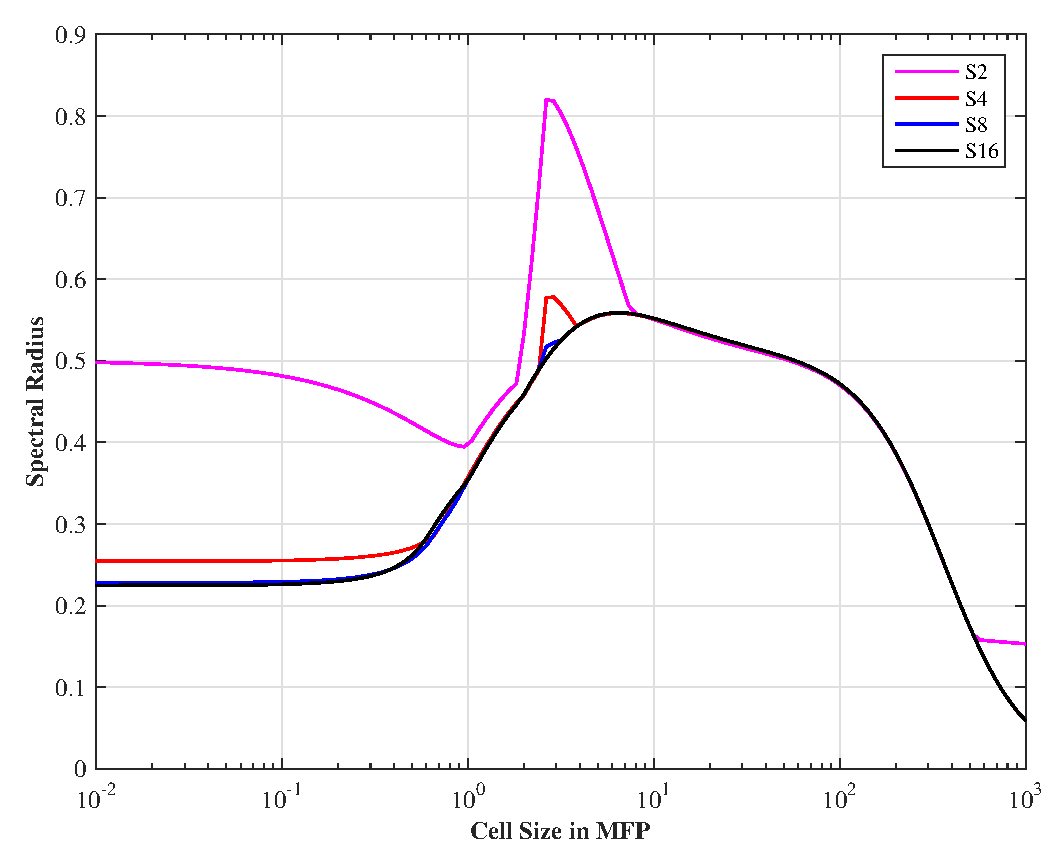
\includegraphics[width=0.975\textwidth]{figures/SI_MIP_hex_C=1_PWLD_LS.eps}
		\caption{$c=1$}
	\end{subfigure}
	\hfill
	\begin{subfigure}[b]{0.49\textwidth}
		\centering
		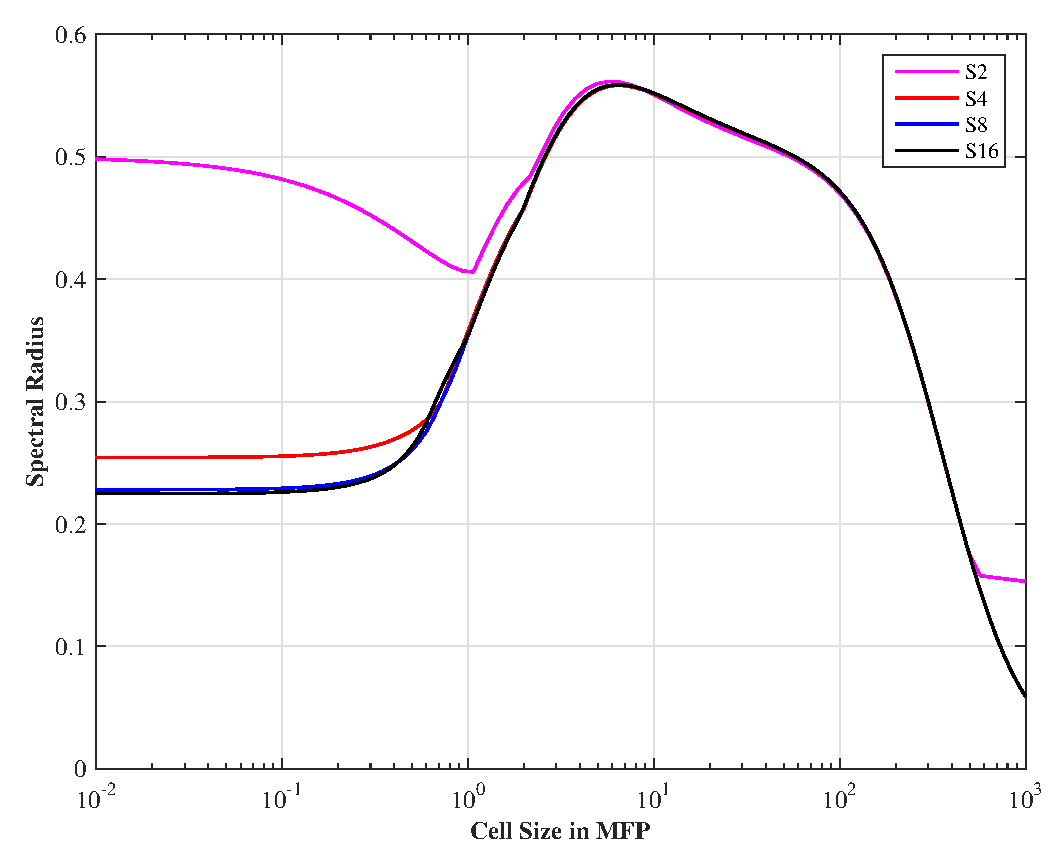
\includegraphics[width=0.975\textwidth]{figures/SI_MIP_hex_C=4_PWLD_LS.eps}
		\caption{$c=4$}
	\end{subfigure}
\caption{Fourier spectral radius of the 3D MIP form for different orders of the level-symmetric quadrature.}
\label{fig::DSA_3D1G_Fourier}
\end{figure}

\begin{figure}
\centering
	\begin{subfigure}[b]{0.49\textwidth}
		\centering
		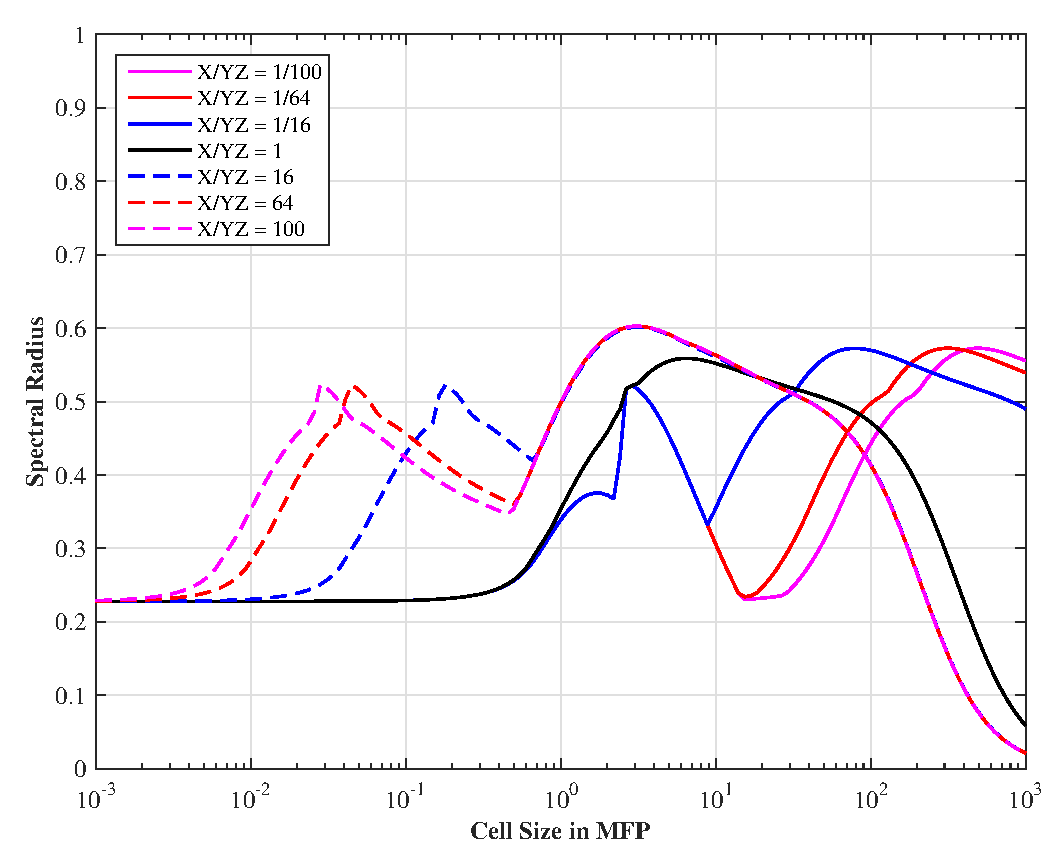
\includegraphics[width=0.975\textwidth]{figures/SI_MIP_hex_AR1.eps}
		\caption{$c=1$}
	\end{subfigure}
	\hfill
	\begin{subfigure}[b]{0.49\textwidth}
		\centering
		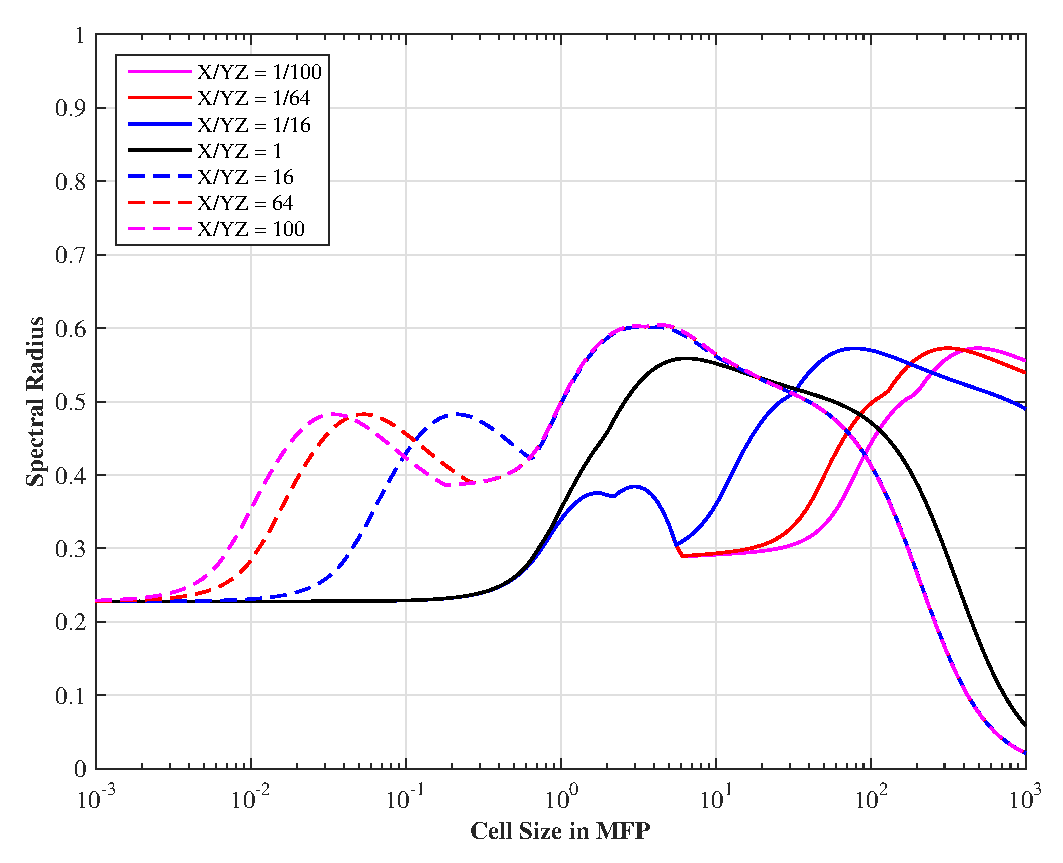
\includegraphics[width=0.975\textwidth]{figures/SI_MIP_hex_AR4.eps}
		\caption{$c=4$}
	\end{subfigure}
\caption{Fourier spectral radii for MIP form with the $S_8$ level-symmetric quadrature on cells with different aspect ratios.}
\label{fig::DSA_3D1G_Fourier_AR}
\end{figure}


\iffalse
\begin{figure}
\centering
	\begin{subfigure}[b]{0.49\textwidth}
		\centering
		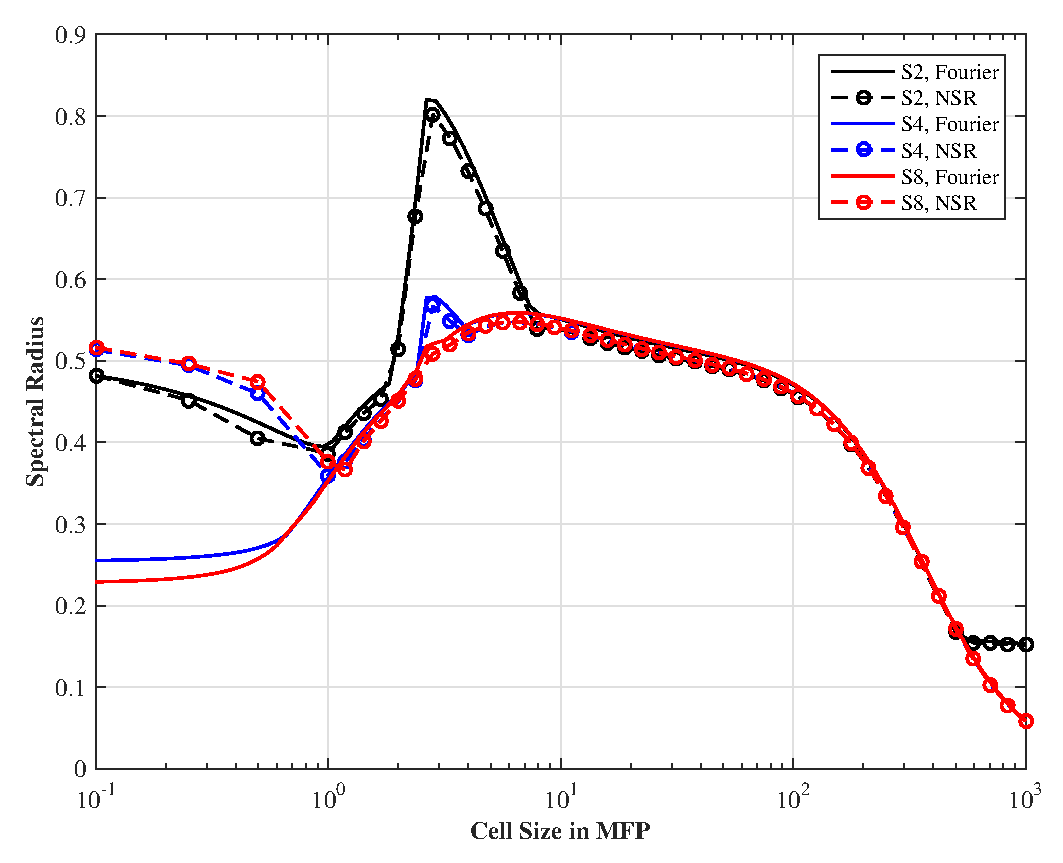
\includegraphics[width=0.975\textwidth]{figures/SI_MIP_hex_C=1_PWLD_LS_wNSR.eps}
	\end{subfigure}
	\hfill
	\begin{subfigure}[b]{0.49\textwidth}
		\centering
		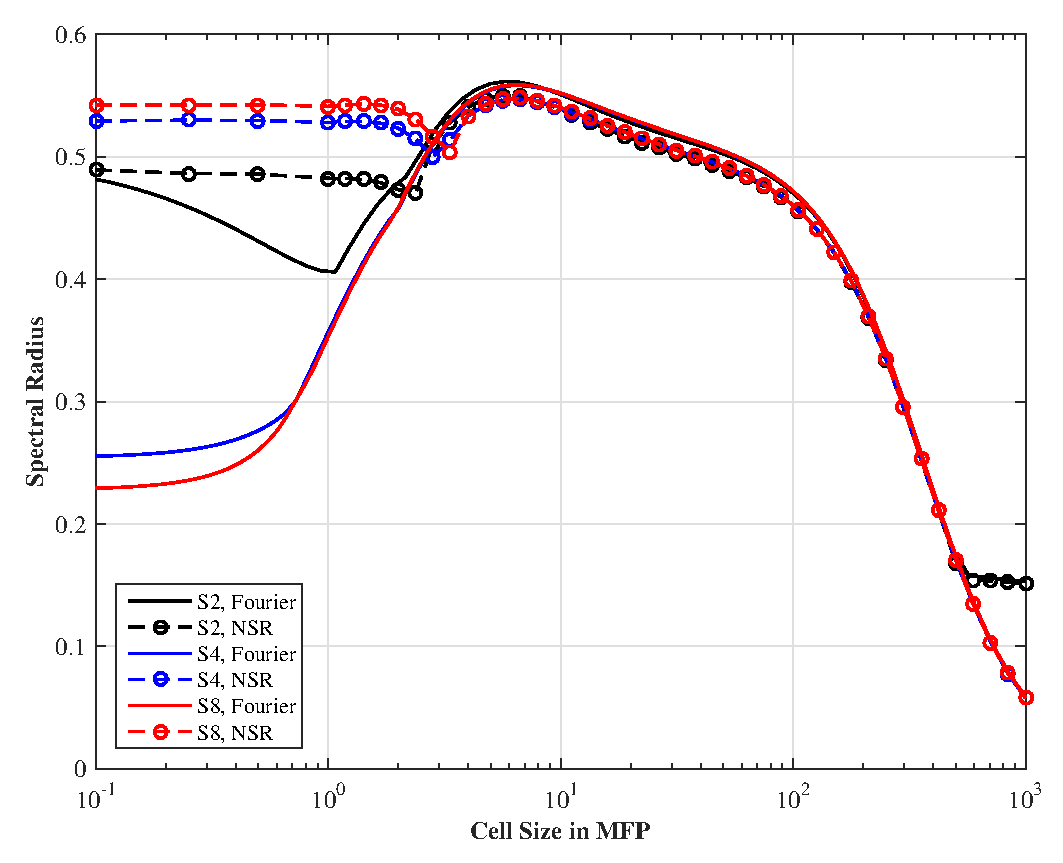
\includegraphics[width=0.975\textwidth]{figures/SI_MIP_hex_C=4_PWLD_LS_wNSR.eps}
	\end{subfigure}
\caption{Comparison between the numerical spectral radii and the theoretical Fourier Analysis spectral radii on the unit cube with $c=1$ (top) and $c=4$ (bottom).}
\label{fig::DSA_3D1G_Fourier_NSR}
\end{figure}
\fi
%%%%%%%%%%%%%%%%%%%%%%%%%%%%%%%%%%%%%%%%%%%%%%%%%%%%%%%%%%%%%%%%%%%%
%%%%%%%%%%%%%%%%%%%%%%%%%%%%%%%%%%%%%%%%%%%%%%%%%%%%%%%%%%%%%%%%%%%%
\section{Timing Analysis} \label{sec::timing}
%%%%%%%%%%%%%%%%%%%%%%%%%%%%%%%%%%%%%%%%%%%%%%%%%%%%%%%%%%%%%%%%%%%%
%%%%%%%%%%%%%%%%%%%%%%%%%%%%%%%%%%%%%%%%%%%%%%%%%%%%%%%%%%%%%%%%%%%%
% Give details of problem analyzed - 3D weak scaling analysis on modified Zerr problem


\begin{figure}
\centering
{
	\begin{subfigure}[b]{\textwidth}
		\centering
		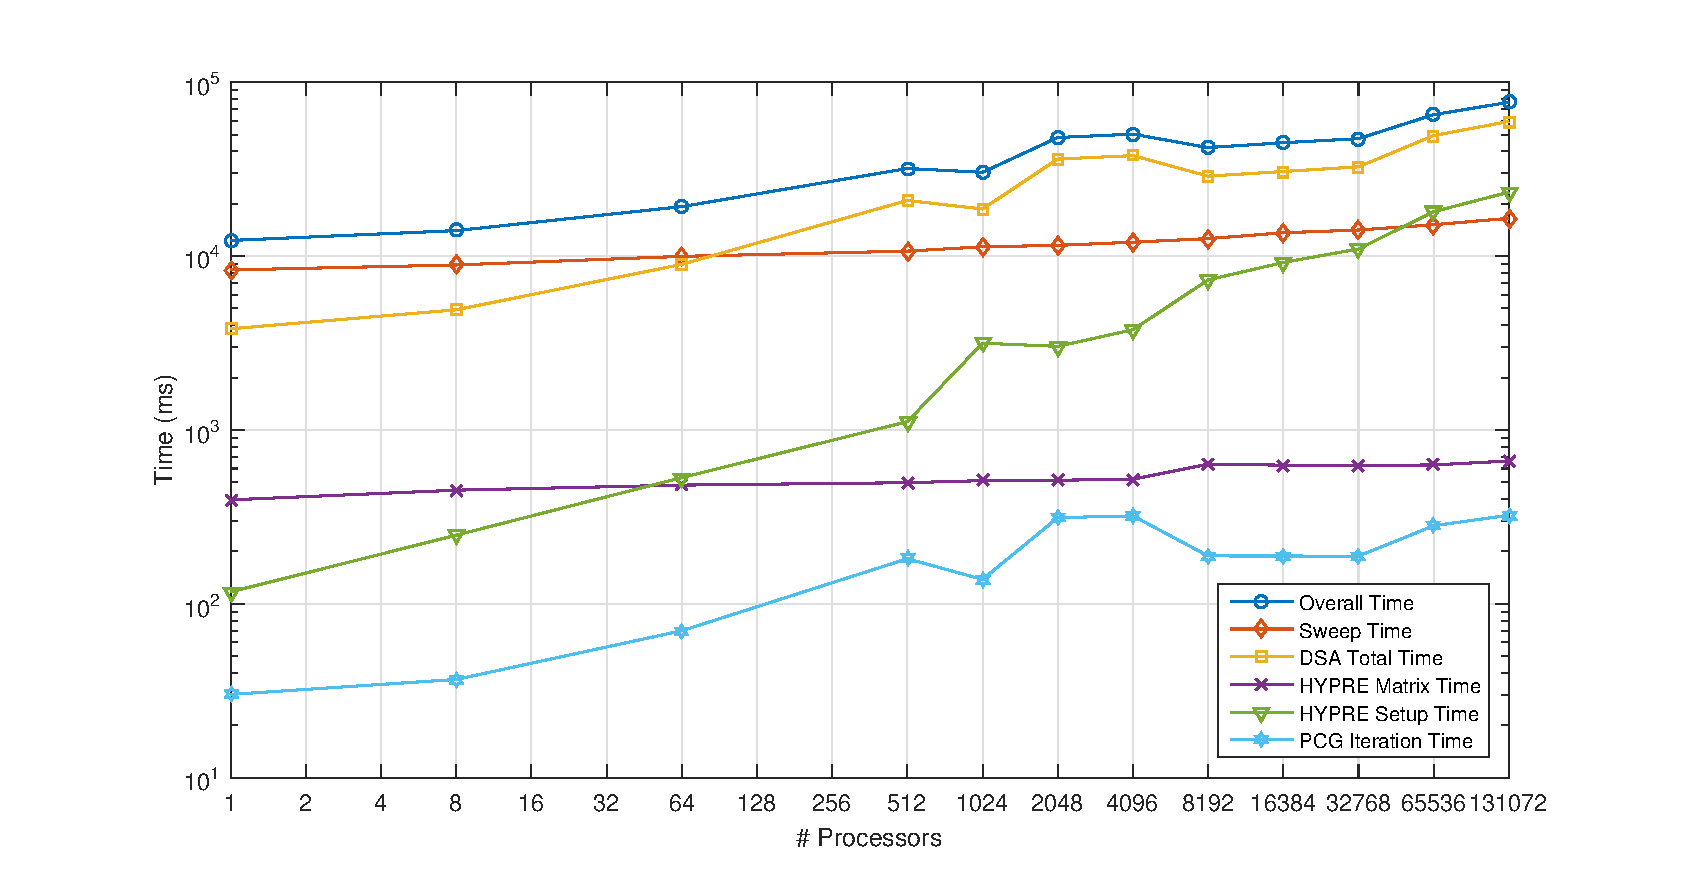
\includegraphics[width=\textwidth]{figures/A128.eps}
		\caption{128 angles and 512 cells per processor}
	\end{subfigure}
}
	\vspace{1cm}
{
	\begin{subfigure}[b]{\textwidth}
		\centering
		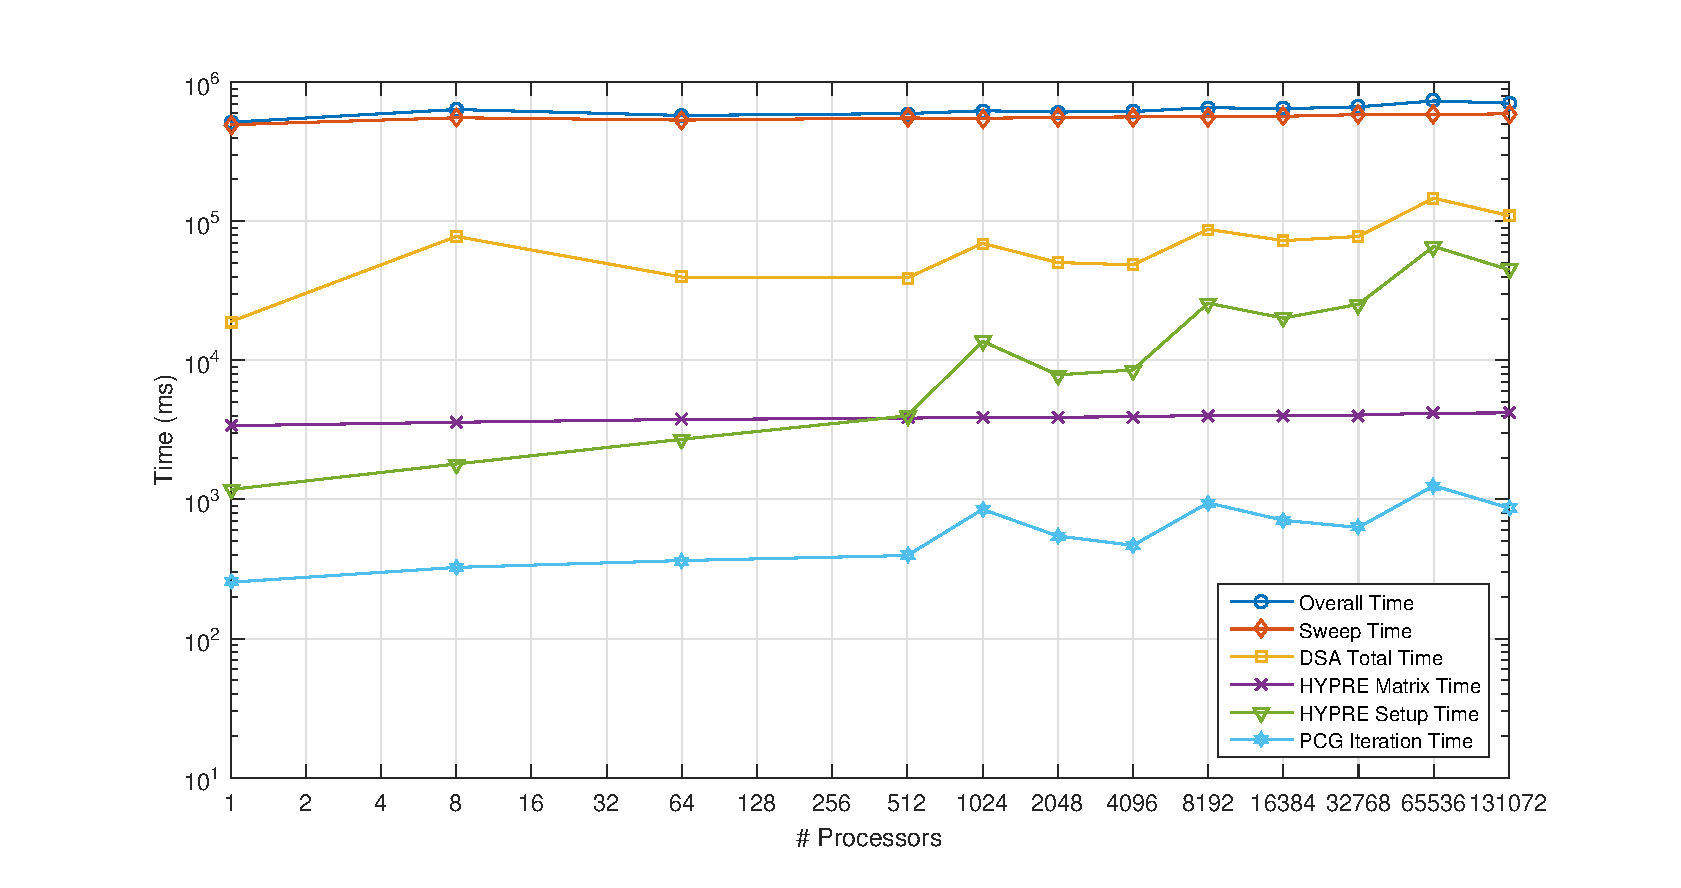
\includegraphics[width=\textwidth]{figures/A2048.eps}
		\caption{2048 angles and 4096 cells per processor}
	\end{subfigure}
}
\caption{Timing data for the MIP DSA implementation in PDT using HYPRE on VULCAN.}
\label{fig::DSA_Scaling_Timing}
\end{figure}

\begin{figure}
\centering
{
	\begin{subfigure}[b]{\textwidth}
		\centering
		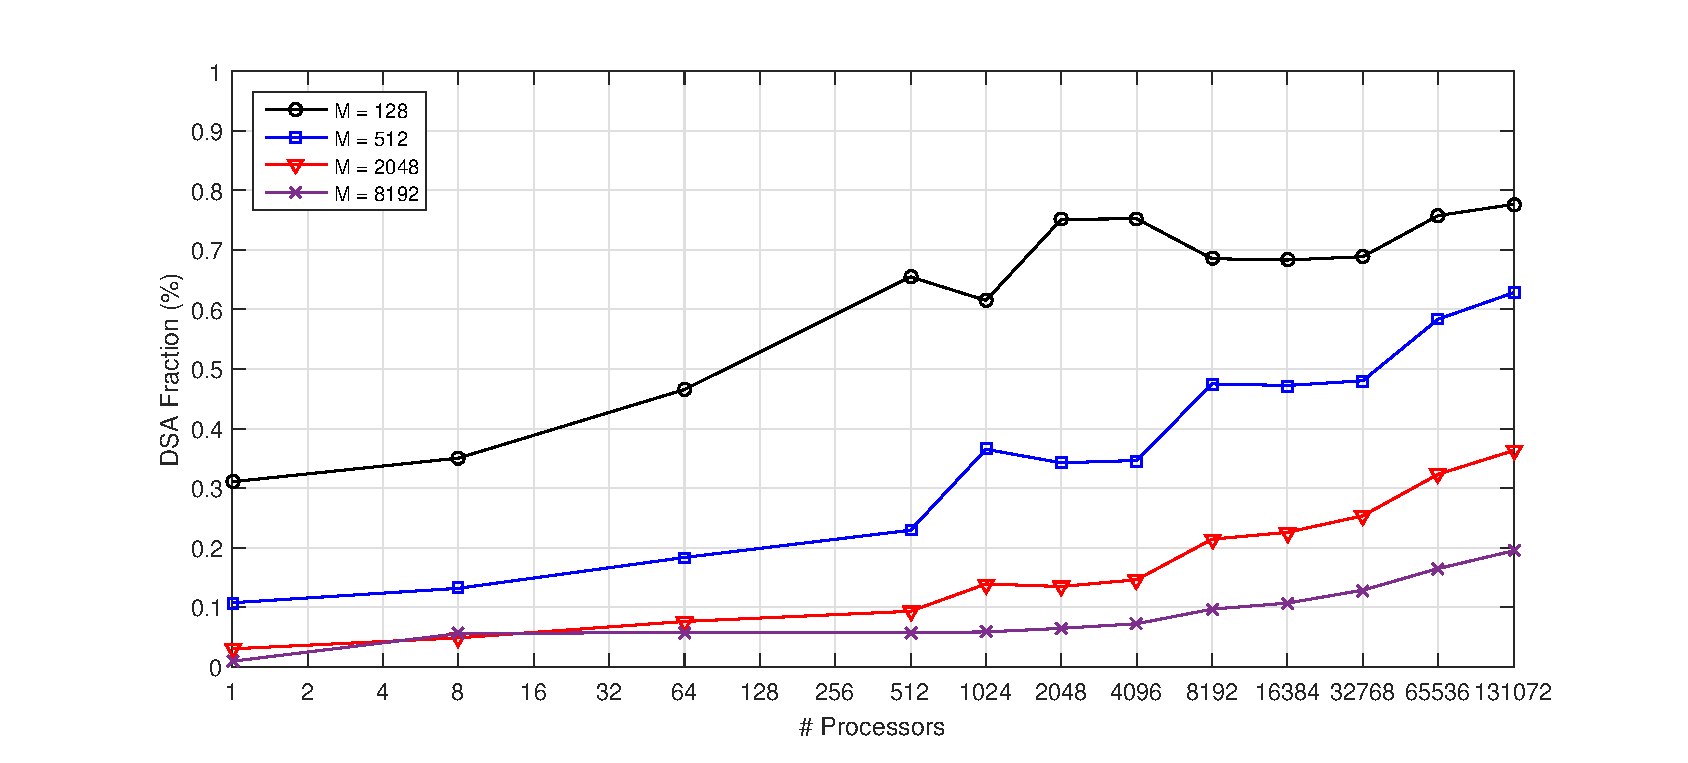
\includegraphics[width=\textwidth]{figures/C512.eps}
		\caption{512 cells per processor}
	\end{subfigure}
}
	\vspace{1cm}
{
	\begin{subfigure}[b]{\textwidth}
		\centering
		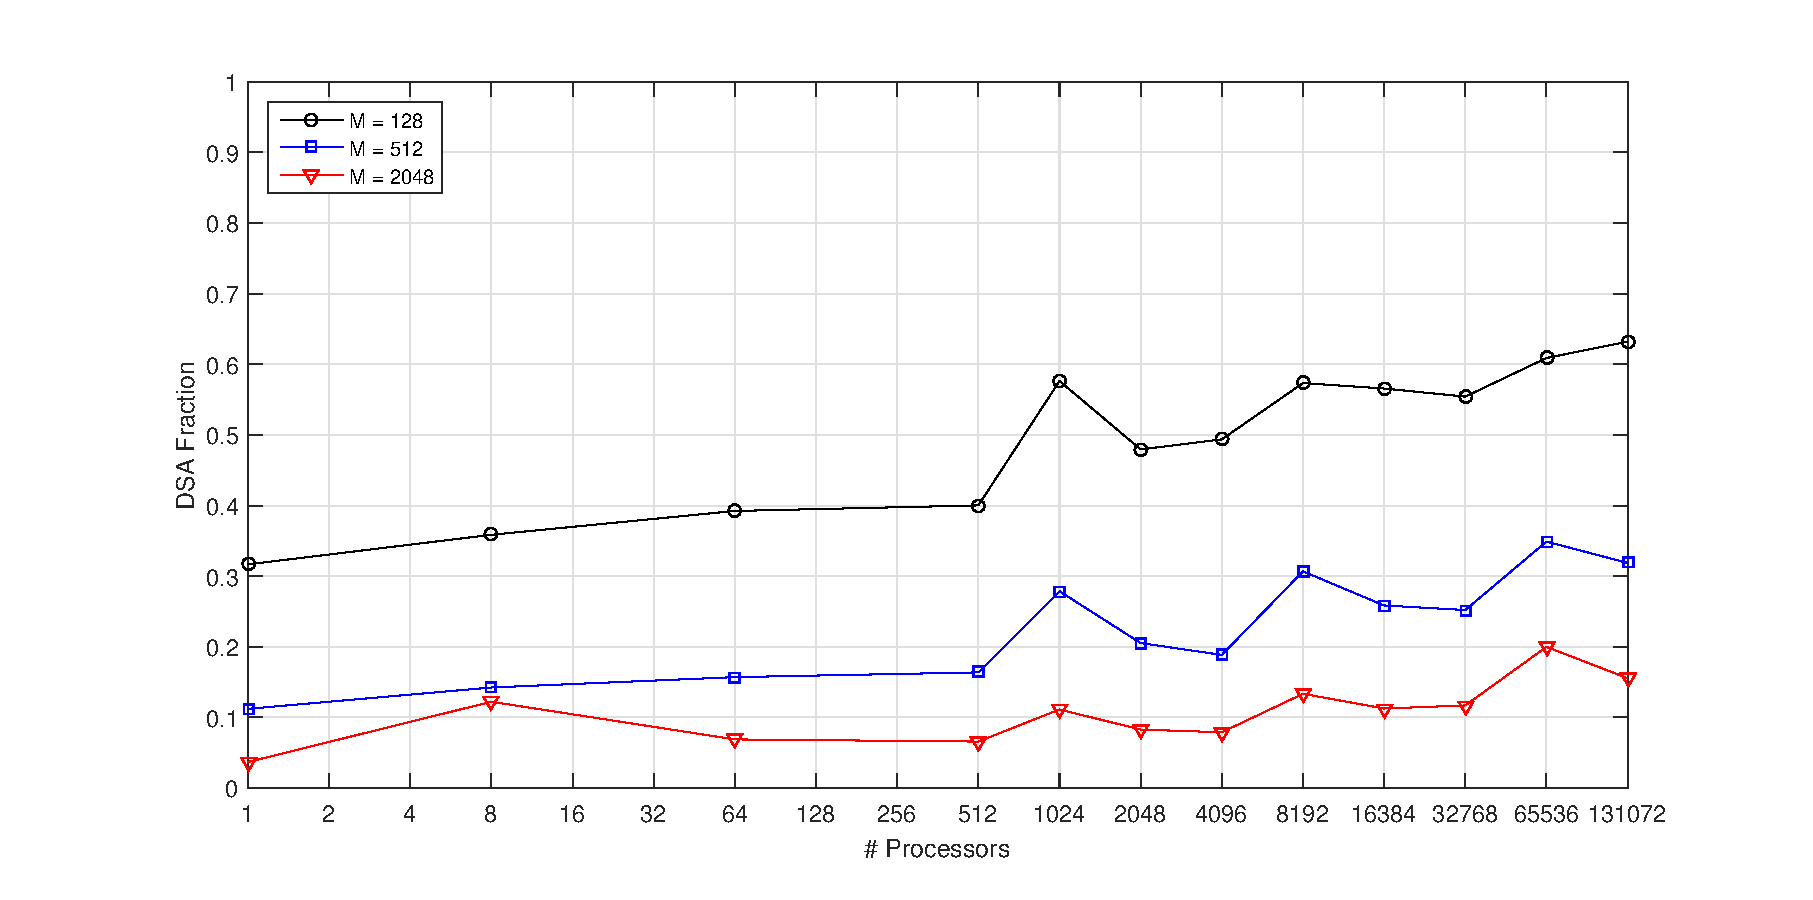
\includegraphics[width=\textwidth]{figures/C4096.eps}
		\caption{4096 cells per processor}
	\end{subfigure}
}
\caption{Fraction of time spent performing DSA based on number of total angles.}
\label{fig::DSA_Scaling_DSAFrac}
\end{figure}

%%%%%%%%%%%%%%%%%%%%%%%%%%%%%%%%%%%%%%%%%%%%%%%%%%%%%%%%%%%%%%%%%%%%
%%%%%%%%%%%%%%%%%%%%%%%%%%%%%%%%%%%%%%%%%%%%%%%%%%%%%%%%%%%%%%%%%%%%
\section{Conclusions} \label{sec::conclusions}
%%%%%%%%%%%%%%%%%%%%%%%%%%%%%%%%%%%%%%%%%%%%%%%%%%%%%%%%%%%%%%%%%%%%
%%%%%%%%%%%%%%%%%%%%%%%%%%%%%%%%%%%%%%%%%%%%%%%%%%%%%%%%%%%%%%%%%%%%

We have 

%%%%%%%%%%%%%%%%%%%%%%%%%%%%%%%%%%%%%%%%%%%%%%%%%%%%%%%%%%%%%%%%%%%%
%%%%%%%%%%%%%%%%%%%%%%%%%%%%%%%%%%%%%%%%%%%%%%%%%%%%%%%%%%%%%%%%%%%%
%%%%%%%%%%%%%%%%%%%%%%%%%%%%%%%%%%%%%%%%%%%%%%%%%%%%%%%%%%%%%%%%%%%%
%%%%%%%%%%%%%%%%%%%%%%%%%%%%%%%%%%%%%%%%%%%%%%%%%%%%%%%%%%%%%%%%%%%%
\pagebreak

\bibliographystyle{elsarticle-num}
\bibliography{references}


\end{document}
